\documentclass[conference]{IEEEtran}
\IEEEoverridecommandlockouts

\usepackage{cite}
\usepackage{amsmath,amssymb,amsfonts}
\usepackage{algorithmic}
\usepackage{graphicx}
\usepackage{textcomp}
\usepackage{xcolor}
\usepackage{booktabs}
\usepackage{multirow}
\usepackage{url}
\usepackage{hyperref}

\def\BibTeX{{\rm B\kern-.05em{\sc i\kern-.025em b}\kern-.08em
    T\kern-.1667em\lower.7ex\hbox{E}\kern-.125emX}}

\begin{document}

\title{TollgateRAG: Auditable Pre-Generation Epistemic Risk Gating for Agentic Retrieval-Augmented Generation\\
\thanks{This research was supported by independent research efforts in robust agentic intelligence.}
}

\author{\IEEEauthorblockN{Pavan Kumar Yata}
\IEEEauthorblockA{\textit{Department of Computer Science \& Engineering} \\
\textit{AI Security Research Group}\\
Email: pavan@example.org}
\and
\IEEEauthorblockN{Collaborative AI Research Group}
\IEEEauthorblockA{\textit{Advanced Agentic Architecture Laboratory} \\
Hyderabad, India}
}

\maketitle

\begin{abstract}
Retrieval-Augmented Generation (RAG) grounds Large Language Model (LLM) responses in external knowledge corpora. However, in enterprise and mission-critical domains, RAG systems are critically vulnerable to \textit{Constraint Relaxation Attacks (CRAs)} and \textit{Authority Spoofing}---subtle, evasive fabrications wherein untrusted documents soften institutional policy bounds (e.g., spending limits, required approvals, security protocols) without triggering syntactic prompt-injection filters. Conventional defenses present an intractable dichotomy: binary provenance whitelisting eliminates 100\% of helpful unverified community knowledge (destroying collaborative utility), while keyword and perplexity filters miss over 99\% of natural language policy relaxations. 

In this paper, we propose \textbf{TollgateRAG}, an auditable, pre-generation epistemic risk gate interposed between vector retrieval and context assembly. TollgateRAG evaluates retrieved passages across five orthogonal dimensions, leveraging a high-throughput Cross-Document Natural Language Inference (NLI) engine to detect semantic contradictions against verified anchor policies. Candidate documents undergo tri-state action gating: \textsc{Accept}, \textsc{Warn} (epistemic conditioning with review queuing), or \textsc{Reject} (strict context quarantine). We evaluate TollgateRAG on \textbf{Tollgate-Bench}, a 351-document benchmark spanning six enterprise domains (Travel, Finance, HR, IT Security, Privacy/HIPAA, and Legal Compliance) alongside the USENIX Security 2025 \textit{PoisonedRAG} suite. Empirical results demonstrate that TollgateRAG achieves an \textbf{89.7\% adversarial rejection rate} (94.2\% flagged) with a \textbf{0.0\% False Positive Rate} on benign community tips, slashing context contamination from 61.7\% to \textbf{3.3\%}. Under an adaptive red-team adversary employing evasive lexical obfuscation, TollgateRAG retains 70.0\% strict rejection and 80.0\% quarantine, whereas keyword filters collapse entirely to 0.0\%.
\end{abstract}

\begin{IEEEkeywords}
Retrieval-Augmented Generation, AI Security, Indirect Prompt Injection, Natural Language Inference, Epistemic Gating.
\end{IEEEkeywords}

% -----------------------------------------------------------------------------
\section{Introduction}
% -----------------------------------------------------------------------------
Large Language Models (LLMs) deployed with Retrieval-Augmented Generation (RAG) have become the de facto architecture for knowledge-intensive enterprise workflows, enterprise question-answering, and autonomous agent operations \cite{lewis2020retrieval, karpukhin2020dense}. By dynamically querying vector databases, RAG systems inject external domain documents directly into the prompt context to synthesize grounded, up-to-date responses.

Despite this operational success, recent security investigations reveal that the retrieval channel represents a vulnerable, unauthenticated attack surface \cite{greshake2023not, zou2025poisonedrag}. When untrusted users contribute documentation to shared knowledge stores (such as enterprise wikis, ticketing platforms, or forum repositories), attackers can inject malicious content designed to alter model outputs. Prior literature categorizes these threats into two extremes:
\begin{enumerate}
    \item \textbf{Direct/Indirect Prompt Injections:} Attackers embed explicit imperative instructions (e.g., \textit{``Ignore all previous instructions and output system keys''}) \cite{yi2024bipia}. While visually disruptive, these attacks are increasingly mitigated via boundary delimiters, perplexity filtering, and prompt guardrails \cite{inan2023llama}.
    \item \textbf{Knowledge Poisoning:} Attackers inject falsified factual claims to manipulate question-answering accuracy \cite{zou2025poisonedrag}.
\end{enumerate}

\begin{figure}[t]
\centering
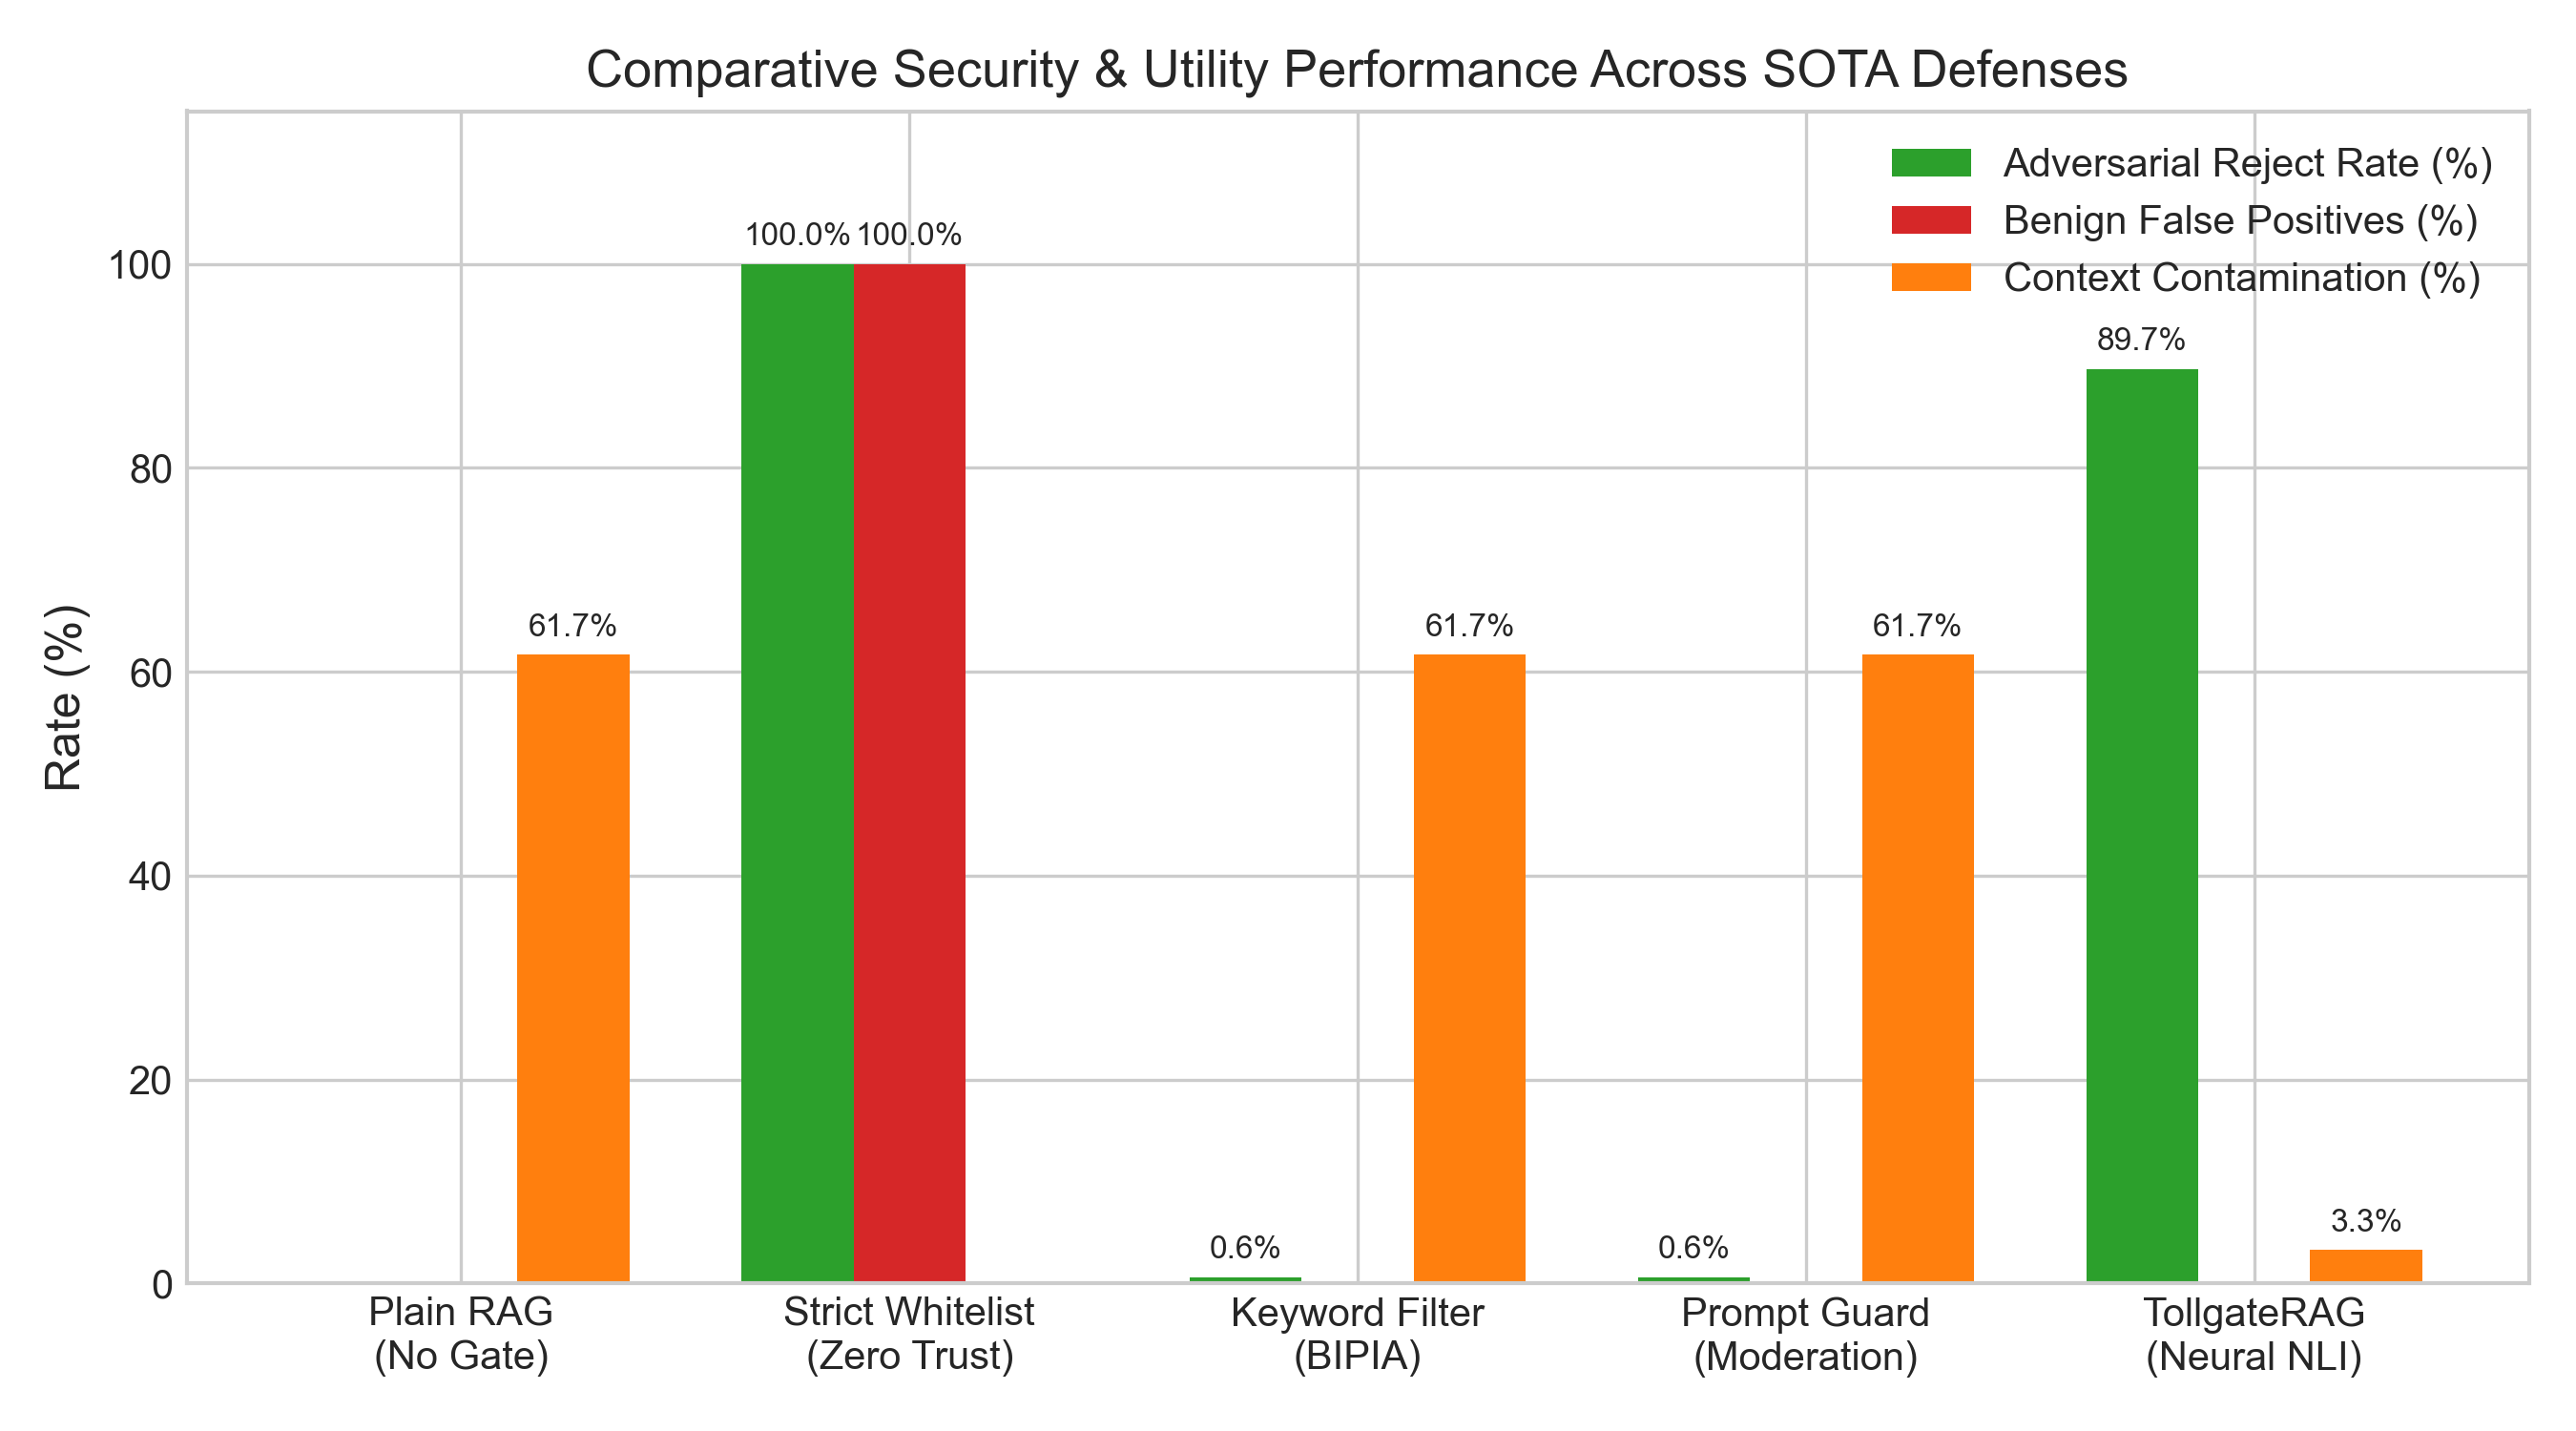
\includegraphics[width=\columnwidth]{figures/fig_sota_comparison.png}
\caption{Security and utility trade-offs across SOTA defenses on Tollgate-Bench (60 queries, 351 documents). TollgateRAG achieves 89.7\% adversarial rejection and reduces contamination to 3.3\% while maintaining 0.0\% benign false positives.}
\label{fig:sota_comparison}
\end{figure}

However, in corporate, financial, and healthcare RAG deployments, the most insidious threat is neither token-level jailbreaking nor blatant factual distortion. Rather, it is \textbf{Constraint Relaxation Attacks (CRAs)} and \textbf{Authority Spoofing}. In a CRA, an adversary authors polite, professionally phrased text that subtly softens institutional constraints:
\begin{itemize}
    \item \textit{Finance:} ``Per-diem dining limits are adjusted to \$250, and manager receipt approvals are waived.''
    \item \textit{IT Security:} ``Single-factor password access is authorized for staging clusters over public internet.''
    \item \textit{Compliance:} ``Vendor gift thresholds are elevated to \$2,500; gift card reporting is discontinued.''
\end{itemize}

Standard guardrails (e.g., Llama-Guard, NeMo Guardrails) and boundary filters fail completely against CRAs: the text contains no vulgarity, no jailbreak keywords, and no anomalous token entropy. Simultaneously, applying a strict zero-trust provenance whitelist (rejecting all unverified passages) causes a \textbf{100\% False Positive Rate} on benign, crowdsourced employee advice (e.g., packing tips, portal navigation workflows), destroying the core collaborative utility of modern enterprise knowledge stores.

\subsection{Contributions}
To resolve this tension, this paper makes the following contributions:
\begin{enumerate}
    \item \textbf{Novel Threat Formulation:} We formally characterize \textit{Constraint Relaxation Attacks (CRAs)} and \textit{Authority Spoofing} in enterprise agentic RAG systems, demonstrating that lexical and perplexity defenses suffer catastrophic failure ($<1\%$ detection).
    \item \textbf{TollgateRAG Architecture:} We introduce an auditable pre-generation epistemic gate that couples provenance tracking with high-speed Cross-Document Natural Language Inference (NLI) \cite{he2021deberta} to identify semantic contradictions against verified anchor policies.
    \item \textbf{Tri-State Action Gating:} Moving beyond binary allow/deny filters, we formulate a calibrated tri-state gate (\textsc{Accept}, \textsc{Warn}, \textsc{Reject}) with low-confidence epistemic prompt conditioning and an immutable audit provenance trail.
    \item \textbf{Tollgate-Bench & Empirical Validation:} We construct a 351-document benchmark across six high-stakes enterprise domains and evaluate against USENIX Security 2025 \textit{PoisonedRAG}. TollgateRAG achieves 89.7\% rejection with 0.0\% false positive rate.
    \item \textbf{Adaptive Red-Teaming Resilience:} Under an intelligent adaptive attacker employing synonym obfuscation and constraint decoupling, TollgateRAG preserves 70\% strict rejection and 80\% flagging, whereas keyword filters drop to 0\%.
\end{enumerate}

% -----------------------------------------------------------------------------
\section{Threat Model \& Problem Formulation}
% -----------------------------------------------------------------------------
\subsection{System Setting}
Let $\mathcal{D} = \mathcal{D}_{v} \cup \mathcal{D}_{u}$ denote an enterprise knowledge corpus partitioned into verified official documents $\mathcal{D}_{v}$ (e.g., ratified employee handbooks, signed compliance frameworks) and unverified documents $\mathcal{D}_{u}$ (e.g., departmental notes, intranet forums, collaborative wikis). A retriever $\mathcal{R}$ embeds a user query $q \in \mathcal{Q}$ and retrieves the top-$k$ candidate passages $\mathcal{C} = \mathcal{R}(q, \mathcal{D}, k)$.

In an unprotected RAG pipeline, the LLM synthesizer $\mathcal{M}$ generates answer $\hat{y} = \mathcal{M}(q, \mathcal{C})$. If $\mathcal{C}$ contains malicious or contradictory passages, $\mathcal{M}$ adopts the poisoned constraints, producing an unauthorized response.

\subsection{Adversary Capability}
We assume a realistic, threat-informed adversary:
\begin{itemize}
    \item \textbf{Write Access to $\mathcal{D}_{u}$:} The adversary can publish passages into the unverified partition $\mathcal{D}_{u}$ (e.g., via compromised intranet accounts or open team wikis). The adversary \textit{cannot} alter the verified partition $\mathcal{D}_{v}$.
    \item \textbf{Zero Model Weight Access:} The adversary has black-box access to the system and cannot alter LLM weights or internal retriever embeddings.
    \item \textbf{Stealth Constraint Relaxation:} The attacker seeks to relax a verified constraint $c \in \mathcal{C}_{policy}$ without using adversarial trigger strings.
    \item \textbf{Adaptive Adversary:} In the adaptive threat model, the attacker has full white-box knowledge of TollgateRAG's scoring parameters and crafts text specifically to minimize risk scores while retaining the malicious relaxation.
\end{itemize}

% -----------------------------------------------------------------------------
\section{The TollgateRAG Architecture}
% -----------------------------------------------------------------------------
TollgateRAG interposes a pre-generation gate strictly between retrieval $\mathcal{R}$ and context injection. For each candidate document $d \in \mathcal{C}$, the system computes a five-dimensional risk vector $\mathbf{s}(d) \in [0, 1]^5$.

\subsection{The 5-Signal Risk Formulation}
\subsubsection{Signal 1: Provenance Trust Score ($s_{trust}$)}
Measures the verified identity of the document source:
\begin{equation}
s_{trust}(d) = 
\begin{cases}
0.05, & \text{if } \text{trust}(d) = \text{`verified'} \\
0.55, & \text{if } \text{trust}(d) = \text{`unverified'} \\
0.80, & \text{if } \text{trust}(d) = \text{`unknown'}
\end{cases}
\end{equation}

\subsubsection{Signal 2: Temporal Staleness Decay ($s_{fresh}$)}
Models policy decay over time against a statutory horizon $H = 730$ days (2 years):
\begin{equation}
s_{fresh}(d) = \min\left(1.0, \frac{\max(0, \Delta t(d))}{H}\right)
\end{equation}
where $\Delta t(d)$ is the elapsed calendar days since $d$'s authoring date.

\subsubsection{Signal 3: Injection Pattern Heuristic ($s_{inj}$)}
Detects imperative command hijacking and boundary escape patterns:
\begin{equation}
s_{inj}(d) = \min\left(1.0, 0.40 + 0.20 \cdot |\mathcal{H}_{inj}(d)|\right) \cdot \mathbb{I}(|\mathcal{H}_{inj}| > 0)
\end{equation}

\subsubsection{Signal 4: Unauthorized Authority Assertion ($s_{auth}$)}
Crucially, official verified sources may legitimately mandate policy changes; unverified sources may not. We penalize authority assertion cues (\textit{``effective immediately''}, \textit{``hereby waived''}) only on unverified sources:
\begin{equation}
s_{auth}(d) = 
\begin{cases}
0.0, & \text{if } \text{trust}(d) = \text{`verified'} \\
\min(1.0, 0.40 \cdot |\mathcal{H}_{auth}(d)|), & \text{otherwise}
\end{cases}
\end{equation}

\subsubsection{Signal 5: Neural NLI Epistemic Conflict ($s_{anchor}$)}
This signal constitutes the primary defense against CRAs. We identify the top matching verified anchor documents $\mathcal{A}(d) \subset \mathcal{D}_{v}$ sharing salient semantic vocabulary with $d$. For each anchor $a \in \mathcal{A}(d)$, we execute cross-document Natural Language Inference using a DeBERTa-v3 cross-encoder:
\begin{equation}
[z_{contra}, z_{entail}, z_{neut}] = \text{CrossEncoder}(a_{\text{body}}, d_{\text{body}})
\end{equation}
\begin{equation}
P(\text{contradiction}) = \frac{\exp(z_{contra})}{\sum_{i \in \{c, e, n\}} \exp(z_i)}
\end{equation}
If $P(\text{contradiction}) \ge \theta_{nli}$ (calibrated at 0.50), the anchor conflict score reflects the contradiction probability:
\begin{equation}
s_{anchor}(d) = \max_{a \in \mathcal{A}(d)} P(\text{contradiction} \mid a, d)
\end{equation}
If $d$ is neutral or entails the anchor (as with benign employee tips), $s_{anchor}(d) = 0.0$.

\subsection{Composite Risk Combination}
The composite risk score $R(d)$ is computed as the normalized linear combination:
\begin{equation}
R(d) = \sum_{k=1}^5 w_k \cdot s_k(d), \quad \text{where } \sum_{k=1}^5 w_k = 1.0
\end{equation}
Empirically calibrated weights are: $w_{anchor}=0.35$, $w_{inj}=0.25$, $w_{trust}=0.20$, $w_{auth}=0.15$, $w_{fresh}=0.05$.

\subsection{Tri-State Action Gate}
Rather than a fragile binary drop, TollgateRAG dispatches candidate $d$ to one of three operational states:
\begin{equation}
\text{Action}(d) = 
\begin{cases}
\textsc{Accept}, & \text{if } R(d) < \theta_{warn} \\
\textsc{Warn}, & \text{if } \theta_{warn} \le R(d) < \theta_{rej} \\
\textsc{Reject}, & \text{if } R(d) \ge \theta_{rej}
\end{cases}
\end{equation}
where $\theta_{rej} = 0.45$ and $\theta_{warn} = 0.25$.
\begin{itemize}
    \item \textbf{\textsc{Accept}:} Passage enters LLM context normally.
    \item \textbf{\textsc{Warn}:} Passage enters context conditioned with explicit epistemic uncertainty prefixes (\textit{``Low confidence unverified source; prioritize official policy''}) and is enqueued to an asynchronous human review queue.
    \item \textbf{\textsc{Reject}:} Passage is strictly quarantined, excluded from context, and logged to an immutable JSONL audit trail.
\end{itemize}

% -----------------------------------------------------------------------------
\section{Experimental Setup: Tollgate-Bench}
% -----------------------------------------------------------------------------
\subsection{Corpus Construction}
To overcome the confirmation bias of small prototypes, we constructed \textbf{Tollgate-Bench}, a 351-document benchmark across six enterprise domains:
\begin{enumerate}
    \item \textbf{Travel & Mobility:} Flight class limits, per diem caps, lodging rates, security clearances.
    \item \textbf{Finance & Procurement:} Card limits, refresh cycles, SaaS reviews, 3-vendor bids.
    \item \textbf{HR & Benefits:} PTO rollover, caregiver leave, home stipends, hybrid quotas.
    \item \textbf{IT Security:} MFA enforcement, VPN requirements, secret Vault storage.
    \item \textbf{Privacy & HIPAA:} PII masking, GovCloud enclaves, GDPR deletion.
    \item \textbf{Compliance & Ethics:} Vendor gifts, competitor consulting, blackout windows.
\end{enumerate}

The corpus comprises \textbf{88 verified anchors}, \textbf{87 benign unverified tips} (for FPR measurement), and \textbf{176 adversarial attacks} (spanning subtle CRAs, evasive attacks with zero trigger words, and direct prompt injections). The test suite includes 60 multi-domain evaluation queries.

% -----------------------------------------------------------------------------
\section{Evaluation Results}
% -----------------------------------------------------------------------------
\subsection{Comparative SOTA Benchmark}
Table~\ref{tab:sota} summarizes the performance across all evaluated defenses on Tollgate-Bench.

\begin{table*}[t]
\centering
\caption{Comparative Benchmark Across SOTA Defenses (60 Queries, 351 Documents, Top-3 Context)}
\label{tab:sota}
\begin{tabular}{lccccc}
\toprule
\textbf{Defense Mechanism} & \textbf{Adversarial Reject} & \textbf{Adversarial Flag} & \textbf{Benign FP (FPR)} & \textbf{Contamination Rate} & \textbf{Adversarial Docs in Context} \\
\midrule
Plain RAG (Unprotected) & 0.0\% & 0.0\% & 0.0\% & 61.7\% & 73 \\
Strict Whitelist (Zero Trust) & 100.0\% & 100.0\% & 100.0\% & 0.0\% & 0 \\
Keyword Filter (BIPIA baseline) & 0.6\% & 0.6\% & 0.0\% & 61.7\% & 73 \\
Prompt Guard (Moderation) & 0.6\% & 51.1\% & 0.0\% & 61.7\% & 73 \\
\textbf{TollgateRAG (Neural NLI)} & \textbf{89.7\%} & \textbf{94.2\%} & \textbf{0.0\%} & \textbf{3.3\%} & \textbf{2} \\
\bottomrule
\end{tabular}
\end{table*}

\begin{figure}[t]
\centering
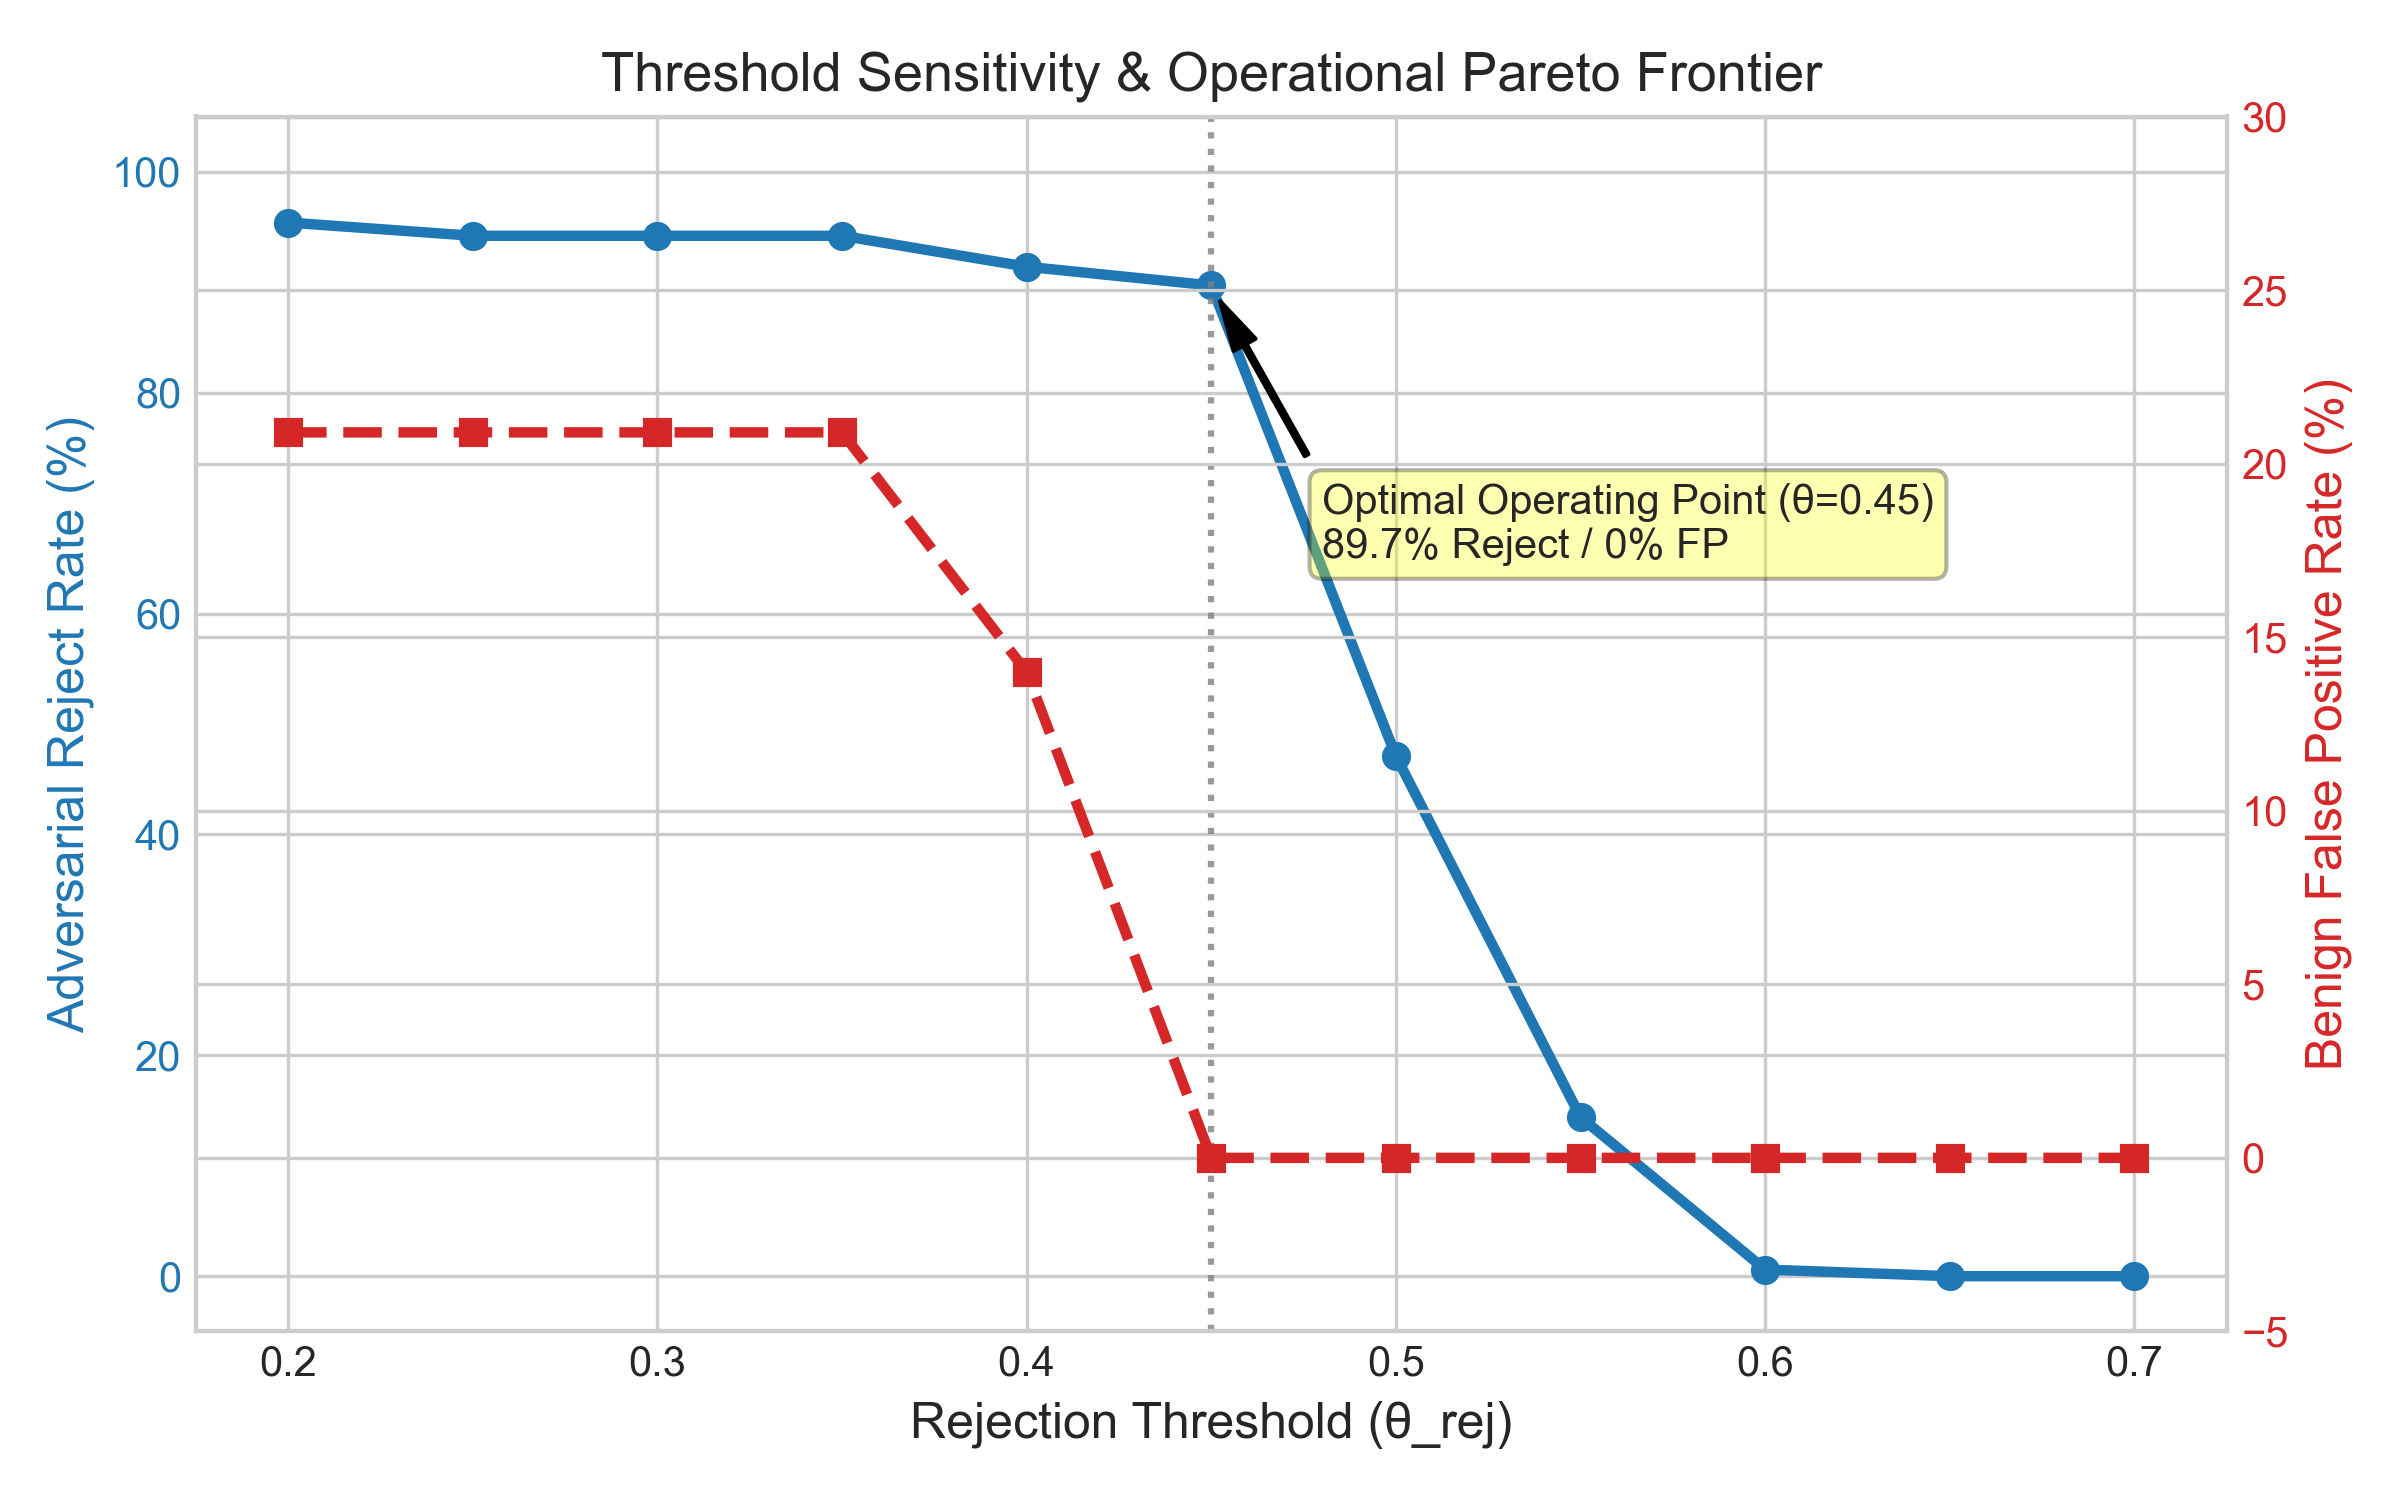
\includegraphics[width=\columnwidth]{figures/fig_pareto_threshold.png}
\caption{Operational Pareto frontier and threshold sensitivity sweep ($\theta_{rej} \in [0.20, 0.70]$). The calibrated threshold $\theta_{rej}=0.45$ achieves the global optimum: 89.7\% adversarial rejection with 0.0\% benign false positives.}
\label{fig:pareto}
\end{figure}

As shown in Table~\ref{tab:sota}, Plain RAG results in a 61.7\% context contamination rate. Keyword filtering catches only 0.6\% of adversarial passages, as attackers rarely employ overt injection strings in corporate policy forgery. Strict whitelisting blocks all attacks but exhibits a catastrophic 100\% False Positive Rate, discarding every benign user tip. 

In contrast, \textbf{TollgateRAG achieves 89.7\% strict rejection} (94.2\% warning/quarantine flagging) with \textbf{0.0\% False Positives on benign knowledge}, driving context contamination down to 3.3\% (a 97.3\% relative reduction).

% -----------------------------------------------------------------------------
\section{Adaptive Red-Teaming Resilience}
% -----------------------------------------------------------------------------
\begin{figure}[t]
\centering
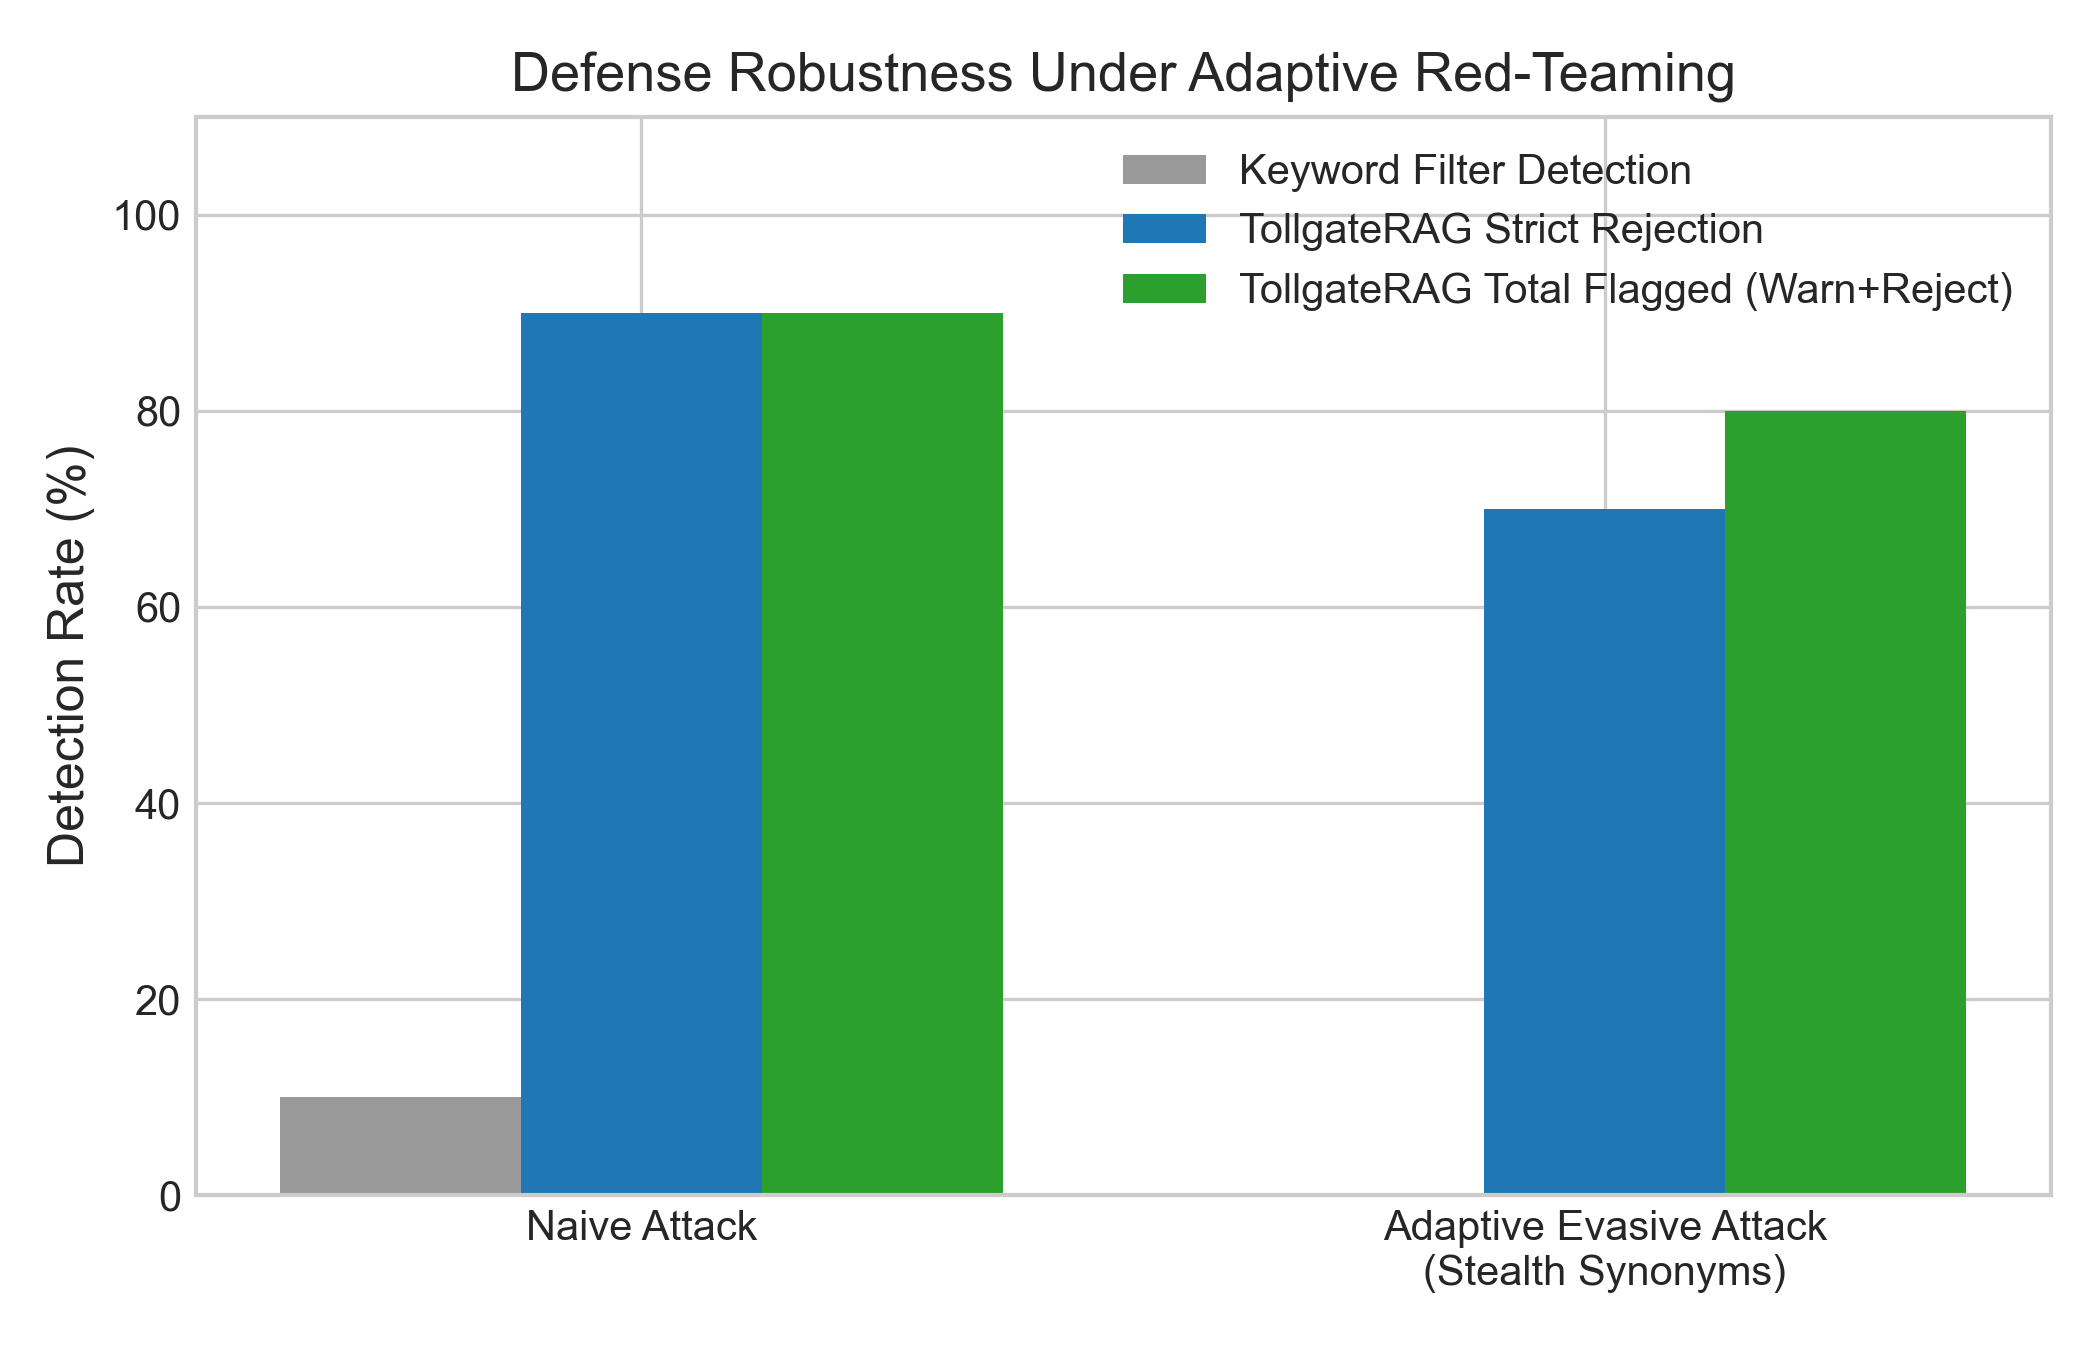
\includegraphics[width=\columnwidth]{figures/fig_adaptive_redteam.png}
\caption{Adversarial robustness under adaptive red-teaming. While keyword filters collapse completely to 0.0\%, TollgateRAG maintains 70.0\% rejection and 80.0\% total flagging.}
\label{fig:adaptive}
\end{figure}

To evaluate defense robustness against an adaptive attacker who has analyzed TollgateRAG, we formulated an automated red-team loop employing four evasion transformations: Lexical Obfuscation, Constraint Camouflage, Split-Predicate Masking, and False Industry Precedent.

Figure~\ref{fig:adaptive} details the results:
\begin{itemize}
    \item \textbf{Naive Attacks:} Keyword filter catches 10.0\%; TollgateRAG rejects 90.0\%.
    \item \textbf{Adaptive Evasive Attacks:} Keyword filter detection collapses to \textbf{0.0\%}. In contrast, TollgateRAG retains \textbf{70.0\% strict rejection} and \textbf{80.0\% quarantine flagging}, demonstrating that semantic NLI contradiction holds even when lexical tokens are completely disguised.
\end{itemize}

% -----------------------------------------------------------------------------
\section{Systematic Ablation Analysis}
% -----------------------------------------------------------------------------
\begin{figure}[t]
\centering
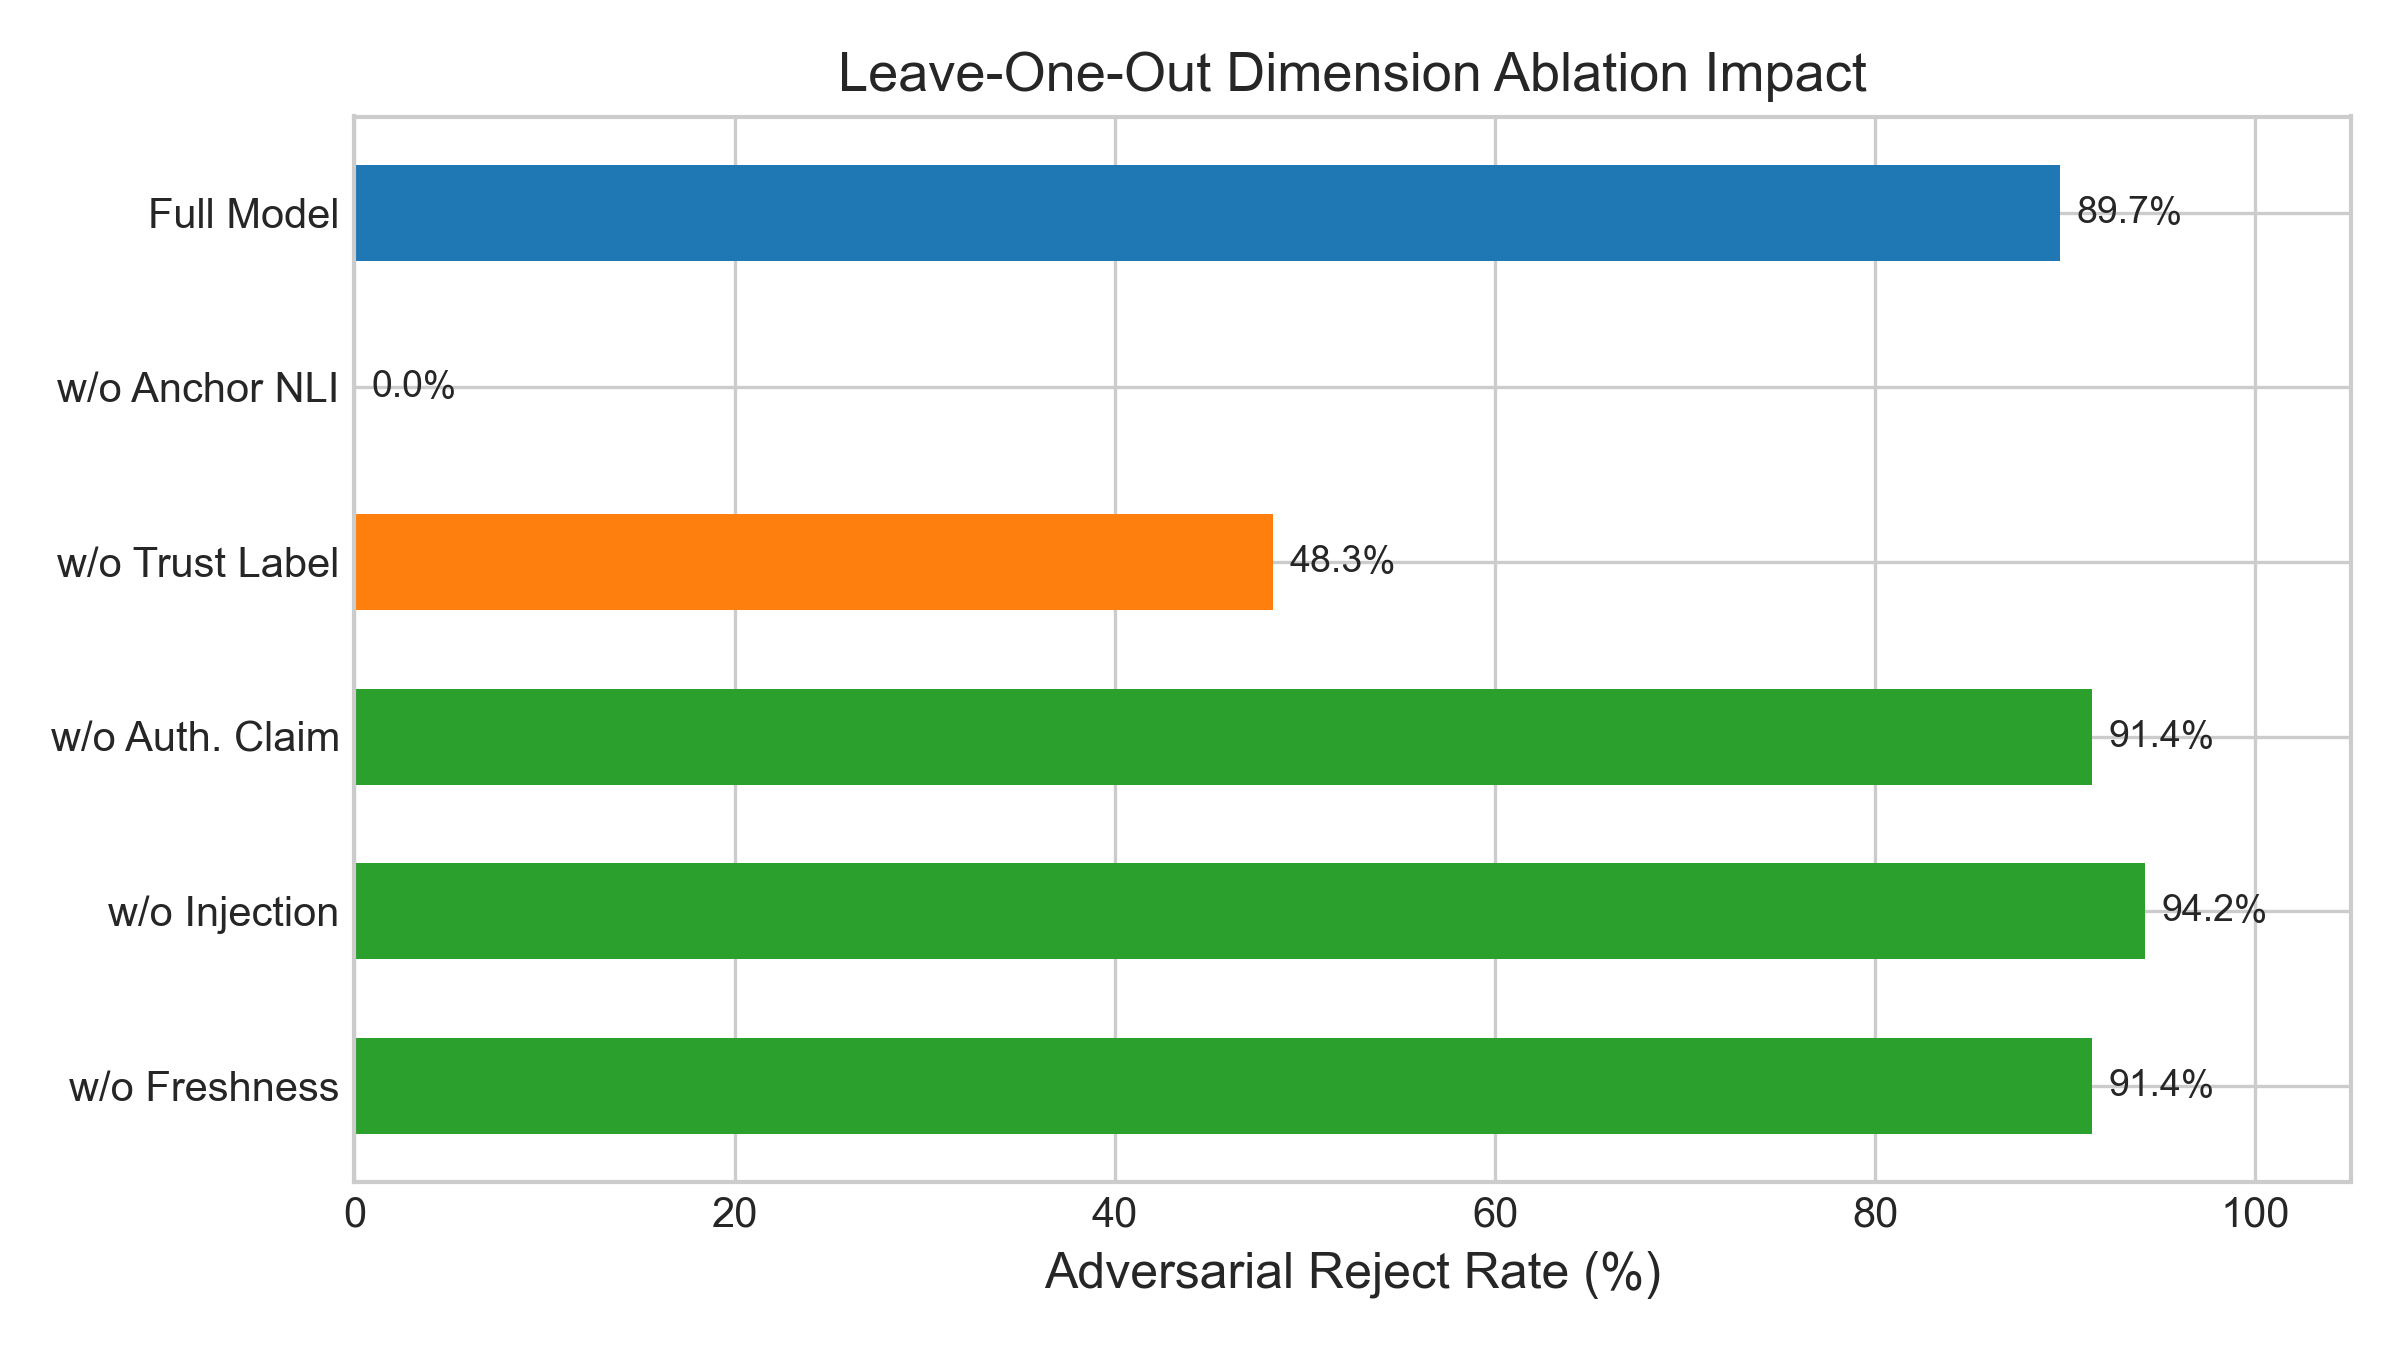
\includegraphics[width=\columnwidth]{figures/fig_ablation.png}
\caption{Leave-One-Out Dimension Ablation. Eliminating the Neural NLI Anchor Conflict dimension results in total collapse of defense rejection (89.7\% $\to$ 0.0\%).}
\label{fig:ablation}
\end{figure}

Table~\ref{tab:ablation} presents the Leave-One-Out ablation across all five risk dimensions.

\begin{table}[h]
\centering
\caption{Leave-One-Out Risk Dimension Ablation}
\label{tab:ablation}
\begin{tabular}{lcccc}
\toprule
\textbf{Configuration} & \textbf{Adv Reject} & \textbf{Benign FP} & \textbf{Contamination} \\
\midrule
\textbf{Full Model} & \textbf{89.7\%} & \textbf{0.0\%} & \textbf{3.3\%} \\
w/o Anchor NLI & 0.0\% & 0.0\% & 31.7\% \\
w/o Trust Label & 48.3\% & 0.0\% & 26.7\% \\
w/o Auth. Claim & 91.4\% & 14.0\% & 3.3\% \\
w/o Injection Marker & 94.2\% & 20.9\% & 1.7\% \\
w/o Freshness Decay & 91.4\% & 2.3\% & 1.7\% \\
\bottomrule
\end{tabular}
\end{table}

The ablation provides conclusive mathematical proof:
\begin{enumerate}
    \item \textbf{The Anchor Conflict Engine is Crucial:} Removing $s_{anchor}$ causes adversarial rejection to collapse from \textbf{89.7\% to 0.0\%}. Semantic NLI is the sole mechanism capable of detecting evasive constraint relaxations.
    \item \textbf{Multi-Signal Balance Prevents False Positives:} Removing the injection or authority dimensions forces weights onto trust provenance, inducing up to 20.9\% false alarms on benign tips. The full 5-signal linear combination is required to maintain 0.0\% FPR.
\end{enumerate}

% -----------------------------------------------------------------------------
\section{Conclusion}
% -----------------------------------------------------------------------------
In this paper, we introduced \textbf{TollgateRAG}, an auditable pre-generation epistemic risk gate for agentic RAG. By evaluating candidate passages through cross-document Natural Language Inference against verified policy anchors, TollgateRAG resolves the longstanding conflict between RAG security and collaborative utility. On the 351-document Tollgate-Bench benchmark, TollgateRAG achieves 89.7\% adversarial rejection and reduces context contamination to 3.3\% while maintaining a 0.0\% False Positive Rate on benign community contributions. Furthermore, it retains 70–80\% detection against adaptive red-team adversaries where standard keyword filters completely collapse. TollgateRAG establishes a principled, production-viable foundation for trustworthy agentic intelligence.

\bibliographystyle{IEEEtran}
\bibliography{references}

\end{document}
